\chapter{Design and Implementation}\label{ch:design}
The previous chapter described an abstract differentially private traffic shaping strategy.
We, now, present \sys's traffic shaping tunnel.
In \Cref{sec:tunnel-overview}, we elaborate on the design of our traffic shaping tunnel,  outlining the essential design criteria for a DP shaping tunnel.
Within this context, we introduce a specific design based on a transport-layer proxy architecture.
In \Cref{sec:tunnel-design}, we elaborate on the operations supported by our tunnel design, encompassing tunnel setup and teardown, connection establishment and termination, as well as outbound traffic shaping.
Finally, in \Cref{sec:eval-simulator}, we conclude this chapter by introducing a traffic shaping simulator that simulates the functionality of the outbound traffic shaping component of our tunnel.



\section{Traffic Shaping Tunnel}\label{sec:tunnel-overview}
We start this section by outlining a set of requirements that a tunnel design for differentially-private traffic shaping should fulfill.
A tunnel must address three requirements.
First, it must satisfy DP guarantees. 
For this, the tunnel~must complete DP measurements and prepare shaped packets within each interval, and it must be able to transmit all payload bytes generated from an application within a finite window length (as defined in the DP strategy).
%
Secondly, the payload and dummy bytes in the shaped packets must be indistinguishable to an adversary.
For this, the tunnel should use a secure encryption protocol to encrypt both data and dummy.
Besides that, the payload and dummy bytes must be transmitted through a shared transport layer so that they are identically acknowledged by the receiver and subject to congestion control and loss recovery mechanisms.
%
Finally, the tunnel must provide similar levels of reliability, congestion control, and loss recovery as expected by the application.
\begin{figure}[t]
  \centering
  %  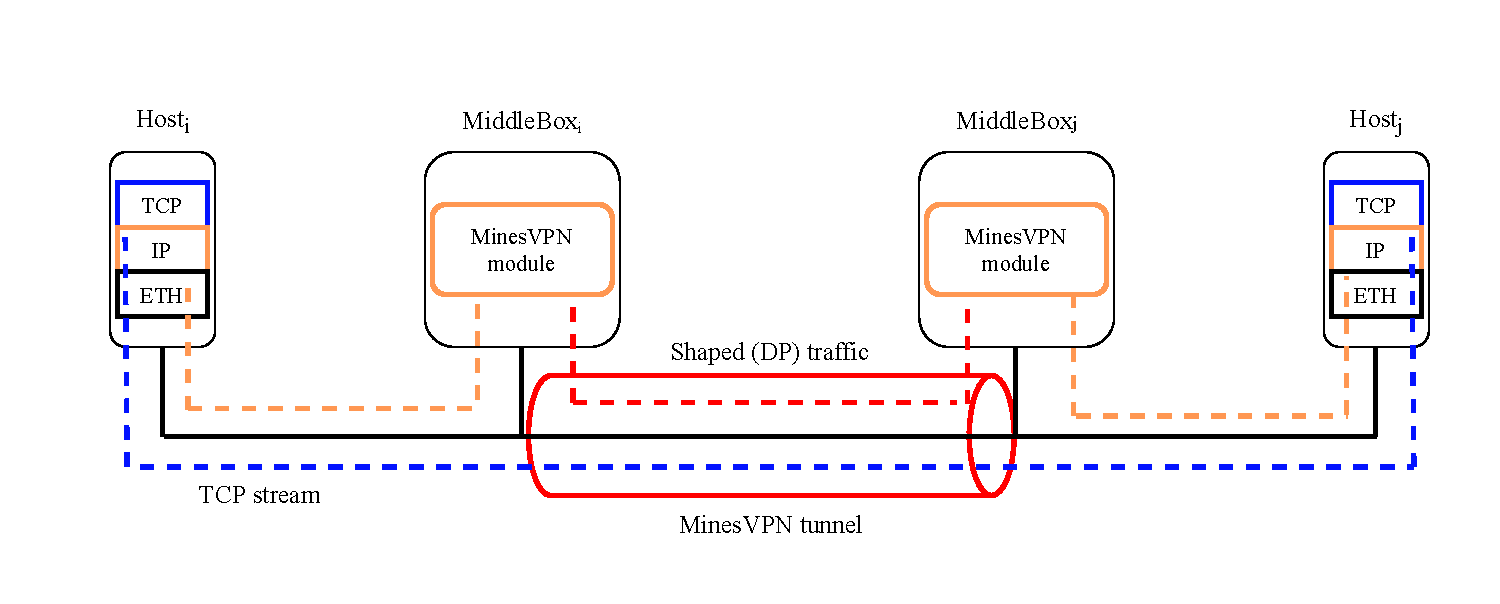
\includegraphics[width=\columnwidth]{figures/Design_highlevel.pdf}
  %  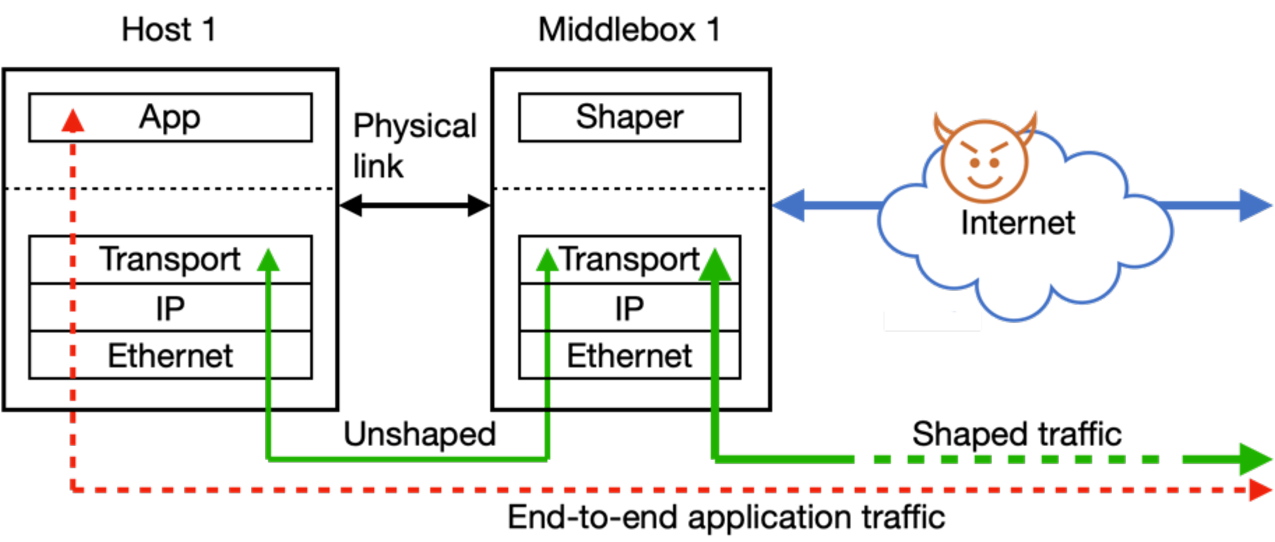
\includegraphics[width=\columnwidth]{figures/minesvpn-overview-half.pdf}
  %  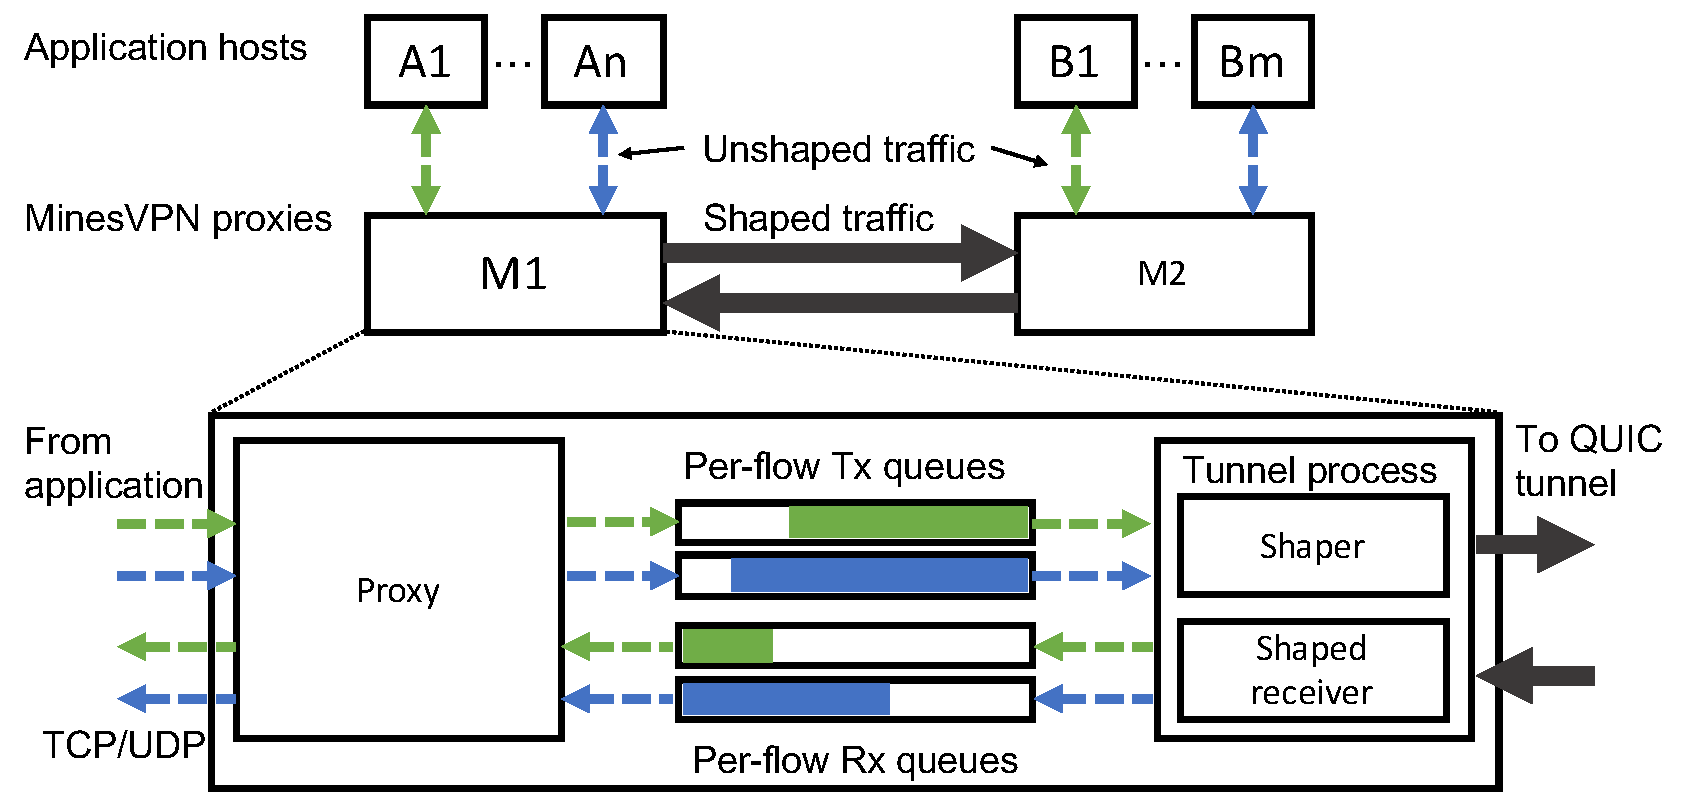
\includegraphics[width=\columnwidth]{figures/minesvpn-arch4.pdf}
  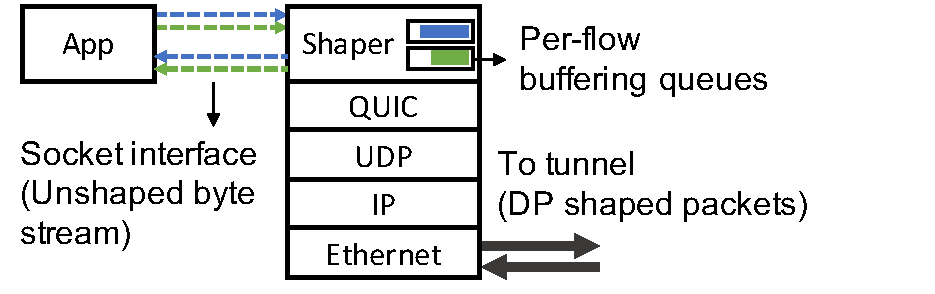
\includegraphics[width=\columnwidth]{figures/design2.pdf}
  \caption{Overview of tunnel design (one endpoint)
      %\am{Update figure}
  }
  \label{fig:minesvpn-overview}
\end{figure}
\Cref{fig:minesvpn-overview} shows the design of one endpoint of {\sys}’s traffic shaping tunnel. A similar endpoint is deployed on the other end of the tunnel.
The shape of the traffic in the tunnel can be configured independently in each direction. The privacy loss in bidirectional streams is the DP composition of the privacy loss in each direction.
A tunnel endpoint consists of a shaping layer (Shaper) on top of QUIC, which in turn runs on top of a standard UDP stack. 
The first requirement should be fulfilled in the implementation of the tunnel, which falls outside the scope of this thesis.
Our design satisfies the second requirement because QUIC deploys encryption for all data transmission, and both data and dummy are sent through a single QUIC connection, ensuring that the receiver identically acknowledges them. 
Finally, QUIC implements congestion control and loss recovery similar to a normal TCP connection, satisfying the third requirement.

It's worth mentioning that aside from QUIC/UDP, {\sys} has the option to utilize a conventional TCP stack as well.
We have specifically chosen QUIC over TCP for the connection between tunnel endpoints because its concept of streams (as discussed in \Cref{sec:background-quic}) allows us to distinguish between dummy and data at the receiver side without the need for additional headers.
The tunnel endpoints establish a bidirectional QUIC connection and generate DP-sized transmit buffers in fixed intervals, which carry payload bytes from one or more application flows.
In the absence of application payload, a tunnel endpoint transmits dummy bytes, which are discarded at the other endpoint.
QUIC encrypts all outbound packets.

{\sys} adopts a transport-layer proxy architecture: each application terminates a connection with the endpoint connected to it.
The application byte stream is sent to the remote application over three piecewise connections: 
(i) between the application and its local tunnel endpoint,
(ii) between the tunnel endpoints, and
(iii) between the remote tunnel endpoint and the remote application.
This ensures only one active congestion control and reliable delivery mechanism in the tunnel and that all bytes are subject to identical mechanisms.
We rely on the transport-layer proxy architecture and discard tunneling TCP through TCP as TCP-in-TCP tunneling causes TCP meltdown~\cite{honda2005tcpovertcp, tcp-meltdown} problem.
In a TCP-in-TCP tunnel, when the network experiences packet loss, the lower-layer TCP initiates packet retransmission to ensure delivery.
However, the upper-layer TCP protocol is unaware of this packet loss and wrongly interprets the increased delay as a sign of a slow network, leading it to decrease the transmission rate.
Consequently, this slower transmission causes the lower-layer TCP protocol to receive acknowledgments too slowly, further mistaking it as packet loss within the network, and thus triggering retransmission.
This repetitive cycle creates a detrimental effect on network performance known as the TCP meltdown problem~\cite{tcp-meltdown}, significantly degrading overall efficiency.
The other option was to use a TCP-in-UDP tunnel. 
This, however, violates the privacy guarantees of {\sys}.
In presence packet loss, the application TCP protocol retransmits data to guarantee data delivery. 
While, the dummy bytes that are injected in the traffic shaping tunnel are not retransmitted, making them observable for adversary. 


\section{Tunnel Design and Operations}\label{sec:tunnel-design}
Now, we describe the fundamental operations that a well-designed {\sys} tunnel must support.
Irrespective of its implementation, a {\sys} tunnel must offer a set of essential functionalities, including tunnel setup and teardown, connection establishment and termination, outbound traffic shaping, and inbound traffic processing. 

\paragraph{Tunnel setup and teardown}
Before applications can communicate with each other, a {\sys} tunnel must be set up between their local tunnel endpoints (as described in \Cref{fig:minesvpn-overview}).
The initiator application can optionally send a configuration message to its local tunnel endpoint with the source and destination IP addresses and ports, and a privacy descriptor.
The privacy descriptor indicates the DP parameters to be used for shaping the tunnel traffic.

Upon receiving a configuration message, the local tunnel endpoint establishes a QUIC connection with the remote tunnel endpoint and configures privacy parameters for each direction.
It also initializes three types of bidirectional~streams in the tunnel: control, dummy, and data streams.
One {\em control stream} is used to transmit messages related to the establishment and termination of a connection between the application endpoints. 
A {\em dummy stream} transmits dummy in QUIC packets in the form of STREAM frames.
We should note that we do not use QUIC's PADDING frames as they do not elicit acknowledgements and hence are distinguishable from STREAM frames \cite{rfc9000}.
The tunnel pre-configures a finite number of data streams, which carry payload bytes from one or more application flows.
When the tunnel is inactive for a period of time, one of the tunnel endpoints initiates a termination sequence and closes all open QUIC streams and the tunnel connection.

\paragraph{Connection establishment and termination}
Once a tunnel is ready, applications can establish and terminate connections with each other, which is mediated by the tunnel.
When the initiator application runs a connection establishment handshake with its local tunnel endpoint, the Shaper maps its flow to a per-flow buffering queue and one of the inactive QUIC data streams in the tunnel, and notifies the remote tunnel endpoint.
The remote tunnel endpoint establishes a connection with the receiver application and maps the receiver application's flow with the data stream.
The connection termination handshake is handled similarly by the tunnel endpoints.
The messages for connection establishment and termination are transmitted over the control stream in the tunnel and shaped according to the tunnel's parameters.

\paragraph{Outbound traffic shaping.}
The Shaper accumulates the outbound bytes of an application flow in a buffering queue before it transmits them in packets whose sizes and timing follow a distribution that guarantees DP.
Within a tunnel, the Shaper transmits bytes from all active flows into a differentially-private packet sequence.
At periodic intervals, called DP measurement intervals, the Shaper performs a DP measurement on the per-flow queues to determine the number of bytes $\qlendp$ to be~transmitted according to the tunnel's DP parameters.
It prepares a {\em shaped buffer} consisting of $\payload$ payload bytes and $\dummy$ dummy bytes, where $\payload$ is the minimum of $\qlendp$ and the application bytes available in the buffering~queues, and $\dummy = \qlendp - \payload$, which may lie between 0 and $\qlendp$.
The Shaper then passes the buffer with the position and length of the padding to QUIC. We simulate the functionality of this component with our traffic shaping simulator in \Cref{sec:eval-simulator}.

QUIC transforms the shaped buffer into one or more STREAM frames based on the
congestion window, the flow window of the receiver endpoint, and the MTU
(maximum transmission unit).
It places the padding bytes into a dummy STREAM frame.
QUIC packages the frames into packets, whose length is at most MTU minus the length of the headers and whose payload is encrypted.
QUIC forwards the packets to the UDP layer, which subsequently transmits the prepared packets as quickly as it can, given the line rate of the NIC.

{\sys} configures the DP measurement interval such that the Shaper can prepare each shaped buffer within an interval.
If the preparation time for a buffer exceeds the interval, the Shaper discards the buffer.
This ensures that the buffering queue length does not grow significantly, which in turn controls the overhead incurred due to DP shaping.
We evaluate the impact of the length of the buffering queue and the DP
measurement interval on privacy guarantees and bandwidth overheads using our simulator in \Cref{ch:evaluation}.

\paragraph{Inbound traffic processing.}
A tunnel endpoint receives shaped packets from the tunnel and applies inverse
processing on each packet.
QUIC receives the packet and
sends an ACK to the sender. Subsequently, it decrypts the packet, discards the
dummy frame, and forwards the payload bytes from the remaining STREAM frames to
the application.

\section{Traffic Shaping Simulator}\label{sec:eval-simulator}
We design and implement a traffic shaping simulator to evaluate the bandwidth overhead and privacy guarantees of {\sys}'s.
The simulator helps users to find parameters of {\sys} shaping mechanism that balance the trade-offs between privacy and overhead according to their requirement.
They can use these parameters in the actual {\sys} system, which we designed in \Cref{sec:tunnel-design} and implemented as part of NetShaper paper \cite{netshaper}.
The simulator specifically simulates the functionality of \emph{Outbound Traffic Shaping} component of a tunnel endpoint to evaluate the privacy and bandwidth overheads of our DP shaping strategy.
The simulator consists of four major components: the Inbound Traffic Processor, responsible for receiving and processing collected traces; the Streaming Application, which emulates the behavior of the application that generated the traffic traces; the Single-Producer Single-Consumer Queue, representing the concept of the buffering queue introduced in \Cref{sec:dp-shaping-definitions} as part of our shaping mechanism; and finally, the Traffic Shaping Module, which implements the core shaping mechanism explained in \Cref{subsec:dp-shaping-mechanism}.


\paragraph{Inbound Traffic Processor}\label{subsubsec:design-sim-inbound}
The simulator takes a PCAP file as the input. 
A PCAP file contains the size and timestamp for every packet that exchanged during a communication session.
To reconstruct the traffic shape from a PCAP file, the simulator discretizes time based on a user defined parameter, \emph{time resolution}.
The \emph{Time resolution} defines the finest level of time granularity upon which the simulator relies.
For instance, if we define \emph{time resolution} as $1ms$, the simulator maps the input trace to a time series, where the $i$\textsuperscript{th} element of time series represent the number of bytes transmitted between the $i$\textsuperscript{th} and the $(i+1)$\textsuperscript{th} millisecond of data transmission (the time series is zero when nothing is sent).
As the data \emph{time resolution} decreases, the simulator more closely replicates the actual shape of the input traffic.
We implement this functionality, as well as preprocessing of the input data, as part of the \texttt{DataProcessor} class in simulator~\cite{netshaper_repo}.



\paragraph{Streaming Application}\label{subsubsec:design-simulator-app}
We develop a simulated application that transmits data based on the time series extracted from PCAP files. 
More precisely, at intervals defined by the \emph{time resolution} of the simulator, the application transmits a quantity of bytes determined by the input time series.
The application continues sending bytes until it either finishes the input traces or it receives a termination signal from the traffic shaping module.
Based on the input trace, simulated application can simulate both server and client side traffic shape.
We implement the simulated application as the \texttt{Application} class in the simulator.

\paragraph{Single-Producer Single-Consumer Queues}\label{subsubsec:design-sim-spsc-queue}
In \Cref{sec:dp-shaping-definitions}, we introduced the \textit{buffering queue} to control the maximum information accessible by an adversary in a predefined time window.
We implement this in the simulator as a simple single-consumer, single-producer queue.
The producer is the streaming application, and
the consumer is our DP traffic shaping module.
The simulated application, as the producer for this queue, pushes a specified number of bytes, based on the input trace, into the queue.
We define a parameter, \emph{shaping interval}, corresponding to the intervals of $T$ seconds we introduced in \Cref{subsec:dp-shaping-mechanism}.
Every $T$ seconds, the shaping module dequeues data with a size determined by
the DP traffic shaping mechanism.



\paragraph{Traffic Shaping Module}
The traffic shaping module is the core part of our simulator where we implement the differentially private traffic shaping mechanism.
Every $T$ seconds, the traffic shaping module determines the number of bytes to be transmitted based on a DP measurement on the size of the application queue, $\qlendp$.
Then, it dequeues $\payload = \min(\qlendp, \qlen)$ from the queue, where $\qlen$ is the number of available bytes in the queue at the measurement time. 
If $\qlendp$ is larger that $\payload$, the traffic shaping module adds $\dummy = \qlendp - \payload$ bytes of dummy data to the transmitted traffic.
We also extend the traffic shaping module to implement constant-rate and Pacer~\cite{mehta2022pacer} traffic shaping to allow comparison between these approaches and {\sys}. 


